% !TeX program = pdflatex
\documentclass[aspectratio=169,10pt]{beamer}

\usepackage[utf8]{inputenc}
\usepackage{amsmath}
\usepackage{booktabs}
\usepackage{tikz}
\usetikzlibrary{arrows.meta,positioning,shapes.geometric}

\usetheme{Madrid}
\usecolortheme{default}
\hypersetup{bookmarks=false}
\setbeamertemplate{navigation symbols}{}
\setbeamertemplate{footline}[frame number]

\definecolor{lungblue}{HTML}{276EF1}
\definecolor{lungteal}{HTML}{009E8E}
\definecolor{lungorange}{HTML}{E77817}
\definecolor{lungred}{HTML}{CF3F36}
\definecolor{lungink}{HTML}{172033}
\definecolor{lungbg}{HTML}{F7F8FB}

\setbeamercolor{title}{fg=lungink}
\setbeamercolor{frametitle}{fg=lungink,bg=white}
\setbeamercolor{structure}{fg=lungblue}
\setbeamercolor{normal text}{fg=lungink,bg=white}
\setbeamercolor{block title}{fg=white,bg=lungblue}
\setbeamercolor{block body}{fg=lungink,bg=lungbg}

\setlength{\parskip}{0.25em}
\linespread{1.03}

\newcommand{\code}[1]{\texttt{\small #1}}
\newcommand{\highlight}[1]{\textcolor{lungblue}{\textbf{#1}}}

\tikzset{
  flowbox/.style={
    draw=lungblue!30,
    fill=white,
    rounded corners=2pt,
    minimum height=1.05cm,
    text width=2.05cm,
    align=center,
    font=\small
  },
  smallflowbox/.style={
    draw=lungblue!30,
    fill=white,
    rounded corners=2pt,
    minimum height=0.95cm,
    text width=1.85cm,
    align=center,
    font=\scriptsize
  },
  flowarrow/.style={-Latex,thick,draw=lungblue},
  feedbackarrow/.style={-Latex,thick,draw=lungteal}
}

\title{LungLogic Single-Lung Flow Control}
\subtitle{PID, Actuator Mapping, Smith Predictor, and Calibration Experiments}
\author{Group Meeting}
\date{}

\begin{document}

\begin{frame}
  \titlepage
\end{frame}

\begin{frame}{Presentation Focus}
  \begin{itemize}
    \item Where is PID used in the current code?
    \item What physical variable does PID control?
    \item What is the actuator?
    \item What does the Smith predictor do in the loop?
    \item What parameters does PID need, and how should they be calibrated?
    \item What parameters does the Smith predictor need, and how should they be calibrated?
  \end{itemize}

  \vspace{0.8em}
  \begin{block}{Key Message}
    PID controls flow rate. The continuous actuator is the PPV40V proportional pinch valve. The Smith predictor only changes the feedback signal seen by PID to compensate pneumatic and sensor delay.
  \end{block}
\end{frame}

\begin{frame}{Closed-Loop Structure}
  \centering
  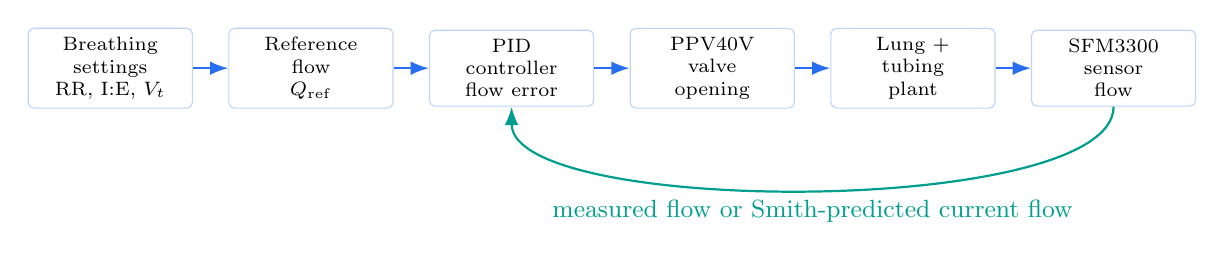
\begin{tikzpicture}[node distance=0.45cm]
    \node[smallflowbox] (settings) {Breathing\\settings\\\scriptsize RR, I:E, $V_t$};
    \node[smallflowbox, right=of settings] (ref) {Reference\\flow\\\scriptsize $Q_{\mathrm{ref}}$};
    \node[smallflowbox, right=of ref] (pid) {PID\\controller\\\scriptsize flow error};
    \node[smallflowbox, right=of pid] (ppv) {PPV40V\\valve\\\scriptsize opening};
    \node[smallflowbox, right=of ppv] (plant) {Lung +\\tubing\\\scriptsize plant};
    \node[smallflowbox, right=of plant] (sensor) {SFM3300\\sensor\\\scriptsize flow};

    \draw[flowarrow] (settings) -- (ref);
    \draw[flowarrow] (ref) -- (pid);
    \draw[flowarrow] (pid) -- (ppv);
    \draw[flowarrow] (ppv) -- (plant);
    \draw[flowarrow] (plant) -- (sensor);

    \draw[feedbackarrow] (sensor.south) .. controls +(0,-1.4) and +(0,-1.4) .. node[below,font=\small,text=lungteal] {measured flow or Smith-predicted current flow} (pid.south);
  \end{tikzpicture}

  \vspace{1.0em}
  \begin{itemize}
    \item Loop objective: make measured flow $Q_{\mathrm{measured}}$ track reference flow $Q_{\mathrm{ref}}$.
    \item Volume is not directly controlled by PID. It is obtained by integrating flow and is used as a phase stop condition.
  \end{itemize}
\end{frame}

\begin{frame}{Where PID Is Used}
  \begin{itemize}
    \item Python simulation: \code{single\_lung\_pid\_gui.py}, \code{PIDController.update()}.
    \item Simulation loop: \code{run\_single\_lung\_simulation()} calls PID during inspiration and expiration.
    \item Hardware path: \code{single\_lung\_hardware\_gui.py} sends $K_p,K_i,K_d$ and related parameters to STM32 through \code{CFG}.
    \item STM32 firmware: \code{updatePID()} runs inside the 100 Hz control loop.
    \item PID is reset at state transitions to avoid carrying integral error across breathing phases.
  \end{itemize}

  \vspace{0.4em}
  \begin{block}{PID Control Law}
    \[
      a=\mathrm{clip}\left(
      a_{\mathrm{ff}}+K_p e+K_i\int e\,dt+K_d d,\ 0,\ 1
      \right)
    \]
  \end{block}
\end{frame}

\begin{frame}{What PID Controls}
  \begin{columns}[T,onlytextwidth]
    \begin{column}{0.48\textwidth}
      \begin{block}{Controlled Variable}
        \[
          Q_{\mathrm{measured}}\rightarrow Q_{\mathrm{ref}}
        \]
        PID controls \highlight{flow rate}, not pressure and not volume directly.
      \end{block}

      \begin{block}{Inspiration Reference}
        \[
          Q_{\mathrm{in,ref}}=0.06\frac{V_{\mathrm{target}}}{T_{\mathrm{fill}}}
        \]
        Default $250$ mL / $1.30$ s:
        \[
          Q_{\mathrm{in,ref}}=11.54\ \mathrm{SLM}
        \]
      \end{block}
    \end{column}
    \begin{column}{0.48\textwidth}
      \begin{block}{Expiration Reference}
        \[
          Q_{\mathrm{out,ref}}=-0.06
          \frac{V_{\mathrm{target}}}{T_{\mathrm{usable,out}}}
        \]
        PID tracks the magnitude of negative expiration flow.
      \end{block}

      \begin{block}{Volume Estimate}
        \[
          V[k]=V[k-1]+Q[k]\frac{1000}{60}\Delta t
        \]
        Volume is used to determine whether the target tidal volume has been reached.
      \end{block}
    \end{column}
  \end{columns}
\end{frame}

\begin{frame}{Actuators}
  \begin{columns}[T,onlytextwidth]
    \begin{column}{0.48\textwidth}
      \begin{block}{Continuous Control Actuator}
        \begin{itemize}
          \item PPV40V proportional pinch valve
          \item PID outputs normalized opening $a\in[0,1]$
          \item $a=0$ means closed, $a=1$ means fully open
        \end{itemize}
      \end{block}

      \begin{block}{Voltage Mapping}
        \[
          U_{\mathrm{cmd}}=5(1-a)
        \]
        \[
          a=1 \Rightarrow 0\ \mathrm{V}\ \mathrm{fully\ open}
        \]
        \[
          a=0 \Rightarrow 5\ \mathrm{V}\ \mathrm{fully\ closed}
        \]
      \end{block}
    \end{column}
    \begin{column}{0.48\textwidth}
      \begin{block}{Direction Selection Actuators}
        \begin{itemize}
          \item Atmosphere solenoid valve
          \item Vacuum solenoid valve
        \end{itemize}
      \end{block}

      \begin{block}{State Machine Output}
        \begin{itemize}
          \item Inspiration: atmosphere valve open, vacuum valve closed
          \item Expiration: atmosphere valve closed, vacuum valve open
          \item Dead time: both directional valves closed
        \end{itemize}
      \end{block}
    \end{column}
  \end{columns}

  \vspace{0.2em}
  \centering
  \highlight{PID continuously modulates PPV40V; solenoid valves only switch the atmosphere/vacuum path.}
\end{frame}

\begin{frame}{Why Smith Predictor Is Needed}
  \begin{itemize}
    \item Pneumatic tubing introduces transport delay.
    \item SFM3300 sensing and signal processing introduce response lag.
    \item If PID directly uses delayed feedback, the response may overshoot, oscillate, or require conservative gains.
    \item The Smith predictor uses the model to estimate current flow, then corrects model error using delayed real measurement.
  \end{itemize}

  \vspace{0.6em}
  \begin{block}{Smith Predictor Feedback Estimate}
    \[
      Q_{\mathrm{feedback}}
      =
      Q_{\mathrm{model,now}}
      +
      g\left(
      Q_{\mathrm{measured,delayed}}
      -
      Q_{\mathrm{model,delayed}}
      \right)
    \]
  \end{block}

  \vspace{0.2em}
  \centering
  The Smith predictor does not replace PID; it provides delay-compensated flow feedback to PID.
\end{frame}

\begin{frame}{Smith Predictor Position}
  \centering
  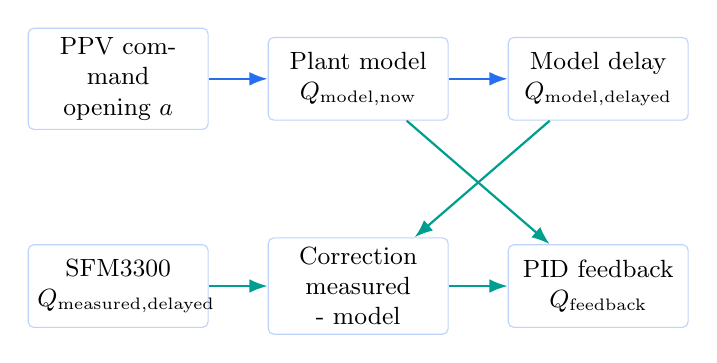
\begin{tikzpicture}[node distance=0.75cm]
    \node[flowbox] (cmd) {PPV command\\opening $a$};
    \node[flowbox, right=of cmd] (model) {Plant model\\$Q_{\mathrm{model,now}}$};
    \node[flowbox, right=of model] (delay) {Model delay\\$Q_{\mathrm{model,delayed}}$};

    \node[flowbox, below=1.45cm of cmd] (sensor) {SFM3300\\$Q_{\mathrm{measured,delayed}}$};
    \node[flowbox, right=of sensor] (corr) {Correction\\measured - model};
    \node[flowbox, right=of corr] (feedback) {PID feedback\\$Q_{\mathrm{feedback}}$};

    \draw[flowarrow] (cmd) -- (model);
    \draw[flowarrow] (model) -- (delay);
    \draw[feedbackarrow] (sensor) -- (corr);
    \draw[feedbackarrow] (delay) -- (corr);
    \draw[feedbackarrow] (model) -- (feedback);
    \draw[feedbackarrow] (corr) -- (feedback);
  \end{tikzpicture}

  \vspace{0.8em}
  \begin{itemize}
    \item Smith disabled: PID feedback = measured flow.
    \item Smith enabled: PID feedback = predicted current flow.
    \item Controller and actuator are unchanged; only the feedback signal changes.
  \end{itemize}
\end{frame}

\begin{frame}{Current Model Parameters}
  \centering
  \begin{block}{Lung and Valve Model}
    \begin{tabular}{lll}
      \toprule
      Parameter & Current value & Meaning \\
      \midrule
      \code{capacity\_ml} & 250 mL & effective lung capacity \\
      \code{tau\_in\_s} & 0.57 s & inspiration time constant \\
      \code{tau\_out\_s} & 0.50 s & expiration time constant \\
      \code{valve\_exponent} & 1.15 & PPV nonlinearity exponent \\
      \code{transport\_delay\_s} & 0.025 s & pneumatic transport delay \\
      \code{sensor\_tau\_s} & 0.020 s & sensor response time constant \\
      \code{sensor\_noise\_slm} & 0.10 SLM & simulated sensor noise \\
      \code{flow\_sign} & 1 & sensor direction convention \\
      \bottomrule
    \end{tabular}
  \end{block}

  \vspace{0.4em}
  \small These are initial values for simulation and early hardware tuning, not final identified parameters.
\end{frame}

\begin{frame}{Current Controller Parameters}
  \begin{columns}[T,onlytextwidth]
    \begin{column}{0.48\textwidth}
      \begin{block}{PID Parameters}
        \begin{tabular}{ll}
          \toprule
          Parameter & Current value \\
          \midrule
          $K_p$ & 0.022 \\
          $K_i$ & 0.16--0.21 \\
          $K_d$ & 0.0 \\
          integral limit & 2.0 \\
          control period & 0.01 s \\
          \bottomrule
        \end{tabular}
      \end{block}
    \end{column}
    \begin{column}{0.48\textwidth}
      \begin{block}{Smith Parameters}
        \begin{tabular}{ll}
          \toprule
          Parameter & Current value \\
          \midrule
          enabled & false by default \\
          delay & 0.025 s \\
          correction gain & 0.85--1.0 \\
          \bottomrule
        \end{tabular}
      \end{block}
    \end{column}
  \end{columns}

  \vspace{0.8em}
  \begin{block}{Code Status}
    PID is active in the flow loop. Smith predictor is implemented and configurable, but disabled by default in the current GUI config.
  \end{block}
\end{frame}

\begin{frame}[shrink=5]{Parameters Needed by PID}
  \begin{columns}[T,onlytextwidth]
    \begin{column}{0.48\textwidth}
      \begin{block}{PID Controller Parameters}
        \begin{itemize}
          \item $K_p$: proportional gain
          \item $K_i$: integral gain
          \item $K_d$: derivative gain
          \item integral limit: anti-windup bound
          \item $\Delta t$: control period
        \end{itemize}
      \end{block}
    \end{column}
    \begin{column}{0.48\textwidth}
      \begin{block}{Feedforward Model Parameters}
        \begin{itemize}
          \item $V_{\max}$: effective capacity
          \item $\tau_{\mathrm{in}}$: inspiration time constant
          \item $\tau_{\mathrm{out}}$: expiration time constant
          \item $\gamma$: valve nonlinearity exponent
        \end{itemize}
      \end{block}
    \end{column}
  \end{columns}

  \vspace{0.4em}
  \begin{block}{Feedforward Opening}
    \[
      a_{\mathrm{ff}}=
      \left(\frac{Q_{\mathrm{ref}}}{Q_{\max}}\right)^{1/\gamma}
    \]
    \[
      Q_{\max,\mathrm{in}}=0.06\frac{V_{\max}-V}{\tau_{\mathrm{in}}},
      \quad
      Q_{\max,\mathrm{out}}=0.06\frac{V}{\tau_{\mathrm{out}}}
    \]
  \end{block}
\end{frame}

\begin{frame}[shrink=5]{PID Calibration Experiments}
  \begin{enumerate}
    \item \textbf{Open-loop PPV step tests}
      \begin{itemize}
        \item Fix PPV opening at 20\%, 40\%, 60\%, 80\%, and 100\%.
        \item Test inspiration and expiration separately.
        \item Record flow, integrated volume, and response time.
      \end{itemize}

    \item \textbf{Closed-loop PI tuning}
      \begin{itemize}
        \item Start with $K_d=0$.
        \item Increase $K_p$ until the response is fast but not strongly oscillatory.
        \item Increase $K_i$ to reduce steady-state flow error and tidal volume error.
      \end{itemize}

    \item \textbf{Multi-condition validation}
      \begin{itemize}
        \item Test different RR, I:E, target volume, and target fill time.
        \item Compare rise time, overshoot, steady-state error, and tidal volume error.
      \end{itemize}
  \end{enumerate}
\end{frame}

\begin{frame}[shrink=8]{Parameters Needed by Smith Predictor}
  \begin{columns}[T,onlytextwidth]
    \begin{column}{0.48\textwidth}
      \begin{block}{Smith-Specific Parameters}
        \begin{itemize}
          \item $L$ or \code{delay\_s}: total delay
          \item $g$ or \code{correction\_gain}: correction gain
          \item \code{enabled}: whether Smith predictor is active
        \end{itemize}
      \end{block}

      \begin{block}{Most Important Parameter}
        \[
          L =
          t_{\mathrm{flow\ response}}
          -
          t_{\mathrm{command}}
        \]
        This is the delay between command change and measured flow response.
      \end{block}
    \end{column}
    \begin{column}{0.48\textwidth}
      \begin{block}{Runtime Signals}
        \begin{itemize}
          \item Current PPV opening $a$
          \item Pneumatic direction
          \item Delayed sensor measurement $Q_{\mathrm{measured,delayed}}$
          \item Current model prediction $Q_{\mathrm{model,now}}$
          \item Delayed model prediction $Q_{\mathrm{model,delayed}}$
        \end{itemize}
      \end{block}

      \begin{block}{Correction Gain Meaning}
        $g=0$: fully trust the model.

        $g=1$: fully apply delayed measurement error correction.

        Too large $g$ may amplify noise or model error.
      \end{block}
    \end{column}
  \end{columns}

  \vspace{0.1em}
  \begin{block}{Note}
    The Smith predictor reuses the first-order lung model already introduced in the PID/feedforward slide.
  \end{block}
\end{frame}

\begin{frame}[shrink=5]{Smith Predictor Calibration Experiments}
  \begin{enumerate}
    \item \textbf{Delay identification}
      \begin{itemize}
        \item Apply a PPV opening step.
        \item Record command timestamp, valve voltage, and SFM3300 flow.
        \item Measure the time from command change to clear flow response to identify \code{delay\_s}.
      \end{itemize}

    \item \textbf{Model-delay alignment}
      \begin{itemize}
        \item Generate $Q_{\mathrm{model,now}}$ using the fitted model.
        \item Delay the model output by $L$ to obtain $Q_{\mathrm{model,delayed}}$.
        \item Compare it against measured $Q_{\mathrm{measured}}$.
      \end{itemize}

    \item \textbf{Smith on/off A-B test}
      \begin{itemize}
        \item Keep control settings, breathing settings, and hardware state unchanged.
        \item Run with Smith predictor disabled and enabled.
        \item Compare overshoot, oscillation, time to target volume, and tidal volume error.
      \end{itemize}
  \end{enumerate}
\end{frame}

\begin{frame}{Basic Calibration Before Hardware Migration}
  \begin{itemize}
    \item \textbf{SFM3300 zero-flow calibration}: close all valves and estimate flow offset and noise.
    \item \textbf{Flow direction calibration}: open atmosphere and vacuum paths separately, verify signs, and set \code{flow\_sign}.
    \item \textbf{PPV40V voltage-flow mapping}: test multiple voltages and confirm 0 V fully open, 5 V fully closed.
    \item \textbf{Inspiration step response}: fit $\tau_{\mathrm{in}}$ and $\gamma$.
    \item \textbf{Expiration step response}: fit $\tau_{\mathrm{out}}$ and verify regulated vacuum range.
    \item \textbf{Safety validation}: emergency stop, flow limit, serial watchdog, and directional valve interlock.
  \end{itemize}
\end{frame}

\begin{frame}{Summary}
  \begin{itemize}
    \item PID is used in the flow feedback loop.
    \item PID controls SFM3300 measured flow so it tracks $Q_{\mathrm{ref}}$.
    \item PID outputs PPV40V proportional pinch valve opening.
    \item Solenoid valves only select the atmosphere or vacuum path.
    \item The Smith predictor estimates current flow and corrects model error using delayed measurement.
    \item PID calibration focuses on $K_p,K_i,K_d$, integral limit, and feedforward model parameters.
    \item Smith calibration focuses on total delay, correction gain, and enabled/disabled comparison.
  \end{itemize}

  \vspace{0.6em}
  \begin{block}{One-Sentence Takeaway}
    State machine chooses pneumatic direction; PID modulates PPV opening; Smith predictor improves feedback timing.
  \end{block}
\end{frame}

\end{document}
